\documentclass[11pt]{article}
\usepackage[T1]{fontenc}
\usepackage[utf8]{inputenc}
\usepackage{lmodern}
\usepackage[margin=1in]{geometry}
\usepackage{amsmath,amssymb,amsthm,mathtools}
\usepackage{graphicx,booktabs,array}
\usepackage{xcolor}
\usepackage[obeyspaces,spaces,hyphens]{url}
\usepackage[colorlinks=true,linkcolor=blue!45!black,citecolor=blue!45!black,urlcolor=blue!45!black]{hyperref}
\usepackage[expansion=false]{microtype}
\hypersetup{pdftitle={Uniform permanence of endotactic reaction networks with measurable rates},
pdfsubject={Endotactic permanence, measurable rates, formal verification}}

\newtheorem{theorem}{Theorem}[section]
\newtheorem{lemma}[theorem]{Lemma}
\newtheorem{proposition}[theorem]{Proposition}
\newtheorem{corollary}[theorem]{Corollary}
\theoremstyle{definition}
\newtheorem{definition}[theorem]{Definition}
\theoremstyle{remark}
\newtheorem{remark}[theorem]{Remark}

\newcommand{\R}{\mathbb R}
\newcommand{\U}{\R_{>0}^{d}}
\newcommand{\B}{\mathcal B}
\newcommand{\abs}[1]{\left|#1\right|}
\newcommand{\norm}[1]{\left\|#1\right\|}
\DeclareMathOperator{\spanR}{span}
\DeclareMathOperator{\atanh}{atanh}
\DeclareMathOperator{\cothh}{coth}
\DeclareMathOperator{\interior}{int}
\DeclareUrlCommand\lean{\urlstyle{tt}}
\setlength{\emergencystretch}{2em}

% Author and affiliation fields are blank.
\title{Uniform permanence of endotactic reaction networks\\with measurable rates}
\author{}
\date{October 8, 2026}

\begin{document}
\maketitle

\begin{abstract}
Let a finite reaction network be endotactic in the sense of Craciun, Nazarov and
Pantea, and let its mass-action rate coefficients be arbitrary measurable functions
of time with values almost everywhere in a fixed box $\prod_e[\underline k_e,\overline k_e]$ with
$\underline k_e>0$. Every positive stoichiometric compatibility
class contains a nonempty compact convex set $K$, depending only on the network,
the box and the class, with the following properties: every positive initial state
has a unique global positive Carath\'eodory solution under every such rate history;
$K$ is invariant under every history; and for every compact set $Q$ of positive
initial states there is one deadline $T_Q$, chosen before the initial state and the
history, after which every solution from $Q$ stays in $K$. This is the
classwise uniform permanence for ordinary endotactic networks with arbitrary
signed real complexes and almost-everywhere bounded measurable histories. In
particular it covers the nonnegative-complex domain of the Extended Permanence
Conjecture of Craciun, Nazarov and Pantea
(Conjecture~1.3 of Johnston, Pantea and Donnell). The proof combines a graph-independent finite affine barrier
construction, imported from recent work of OpenAI on weakly reversible networks,
with a new drift estimate for endotactic networks: at every active barrier normal,
the reaction with the lowest adverse source is dominated by a single positive
witness supplied by endotacticity, and the retained projection lengths give a
margin uniform over the rate box. Trapping in convex plateaux and a finite
iteration across logarithmic scales then yield the absorbing set and the uniform
deadline. The real-complex theorem, including global positive Carath\'eodory
solutions, uniqueness among positive solutions, invariance, compact-initial
uniformity, null-set rate repair and initial-data continuous dependence, is
established by strict Lean~4 checks with the standard axioms only. The positive
periodic-solution and equilibrium corollaries are proved conventionally. A three-species network that is neither weakly reversible
nor strongly endotactic illustrates the kind of explicit certificate the
hypotheses allow: for six independently varying measurable coefficients in
$[1/2,2]$, every solution from $[0.1,10]^3$ lies in $[0.4,2.5]^3$ for all times
$t\ge 347/16<22$, a staged bound whose clocked comparison steps and exact
rational roundings are also machine-checked.
\end{abstract}

\section{Introduction}\label{sec:intro}

A mass-action system assigns to each reaction $y\to y'$ of a finite network a
positive rate coefficient and the monomial flux $k\,x^{y}$; the concentration
vector then obeys $\dot x=\sum k_{y\to y'}x^{y}(y'-y)$~\cite{HornJackson1972,Feinberg1972}.
Two long-standing questions concern the long-time behaviour of positive solutions.
\emph{Persistence} asks that no concentration approach zero along a trajectory;
\emph{permanence} asks for one compact set in the positive stoichiometric
compatibility class that every solution in that class eventually enters and never
leaves~\cite{AngeliDeLeenheerSontag2007,CraciunNazarovPantea2013}. The Global
Attractor Conjecture asserts convergence of every positive trajectory of a
complex-balanced system to the unique positive equilibrium in its stoichiometric
compatibility class. It was proved
for a single linkage class by Anderson~\cite{Anderson2011} and in general by
Craciun~\cite{Craciun2015}; see also~\cite{Pantea2012,GopalkrishnanMillerShiu2014}.
For weakly reversible networks with a single linkage class, permanence was proved
by Boros and Hofbauer~\cite{BorosHofbauer2020}.

Craciun, Nazarov and Pantea~\cite{CraciunNazarovPantea2013} observed that the
property that drives these results is not the graph condition of weak
reversibility but a directional one. A network is \emph{endotactic} if, in every
direction $r\in\R^d$, every reaction whose vector points backwards ($r\cdot\nu_e<0$)
is accompanied by a reaction pointing forwards ($r\cdot\nu_j>0$) whose source lies
strictly lower in that direction ($r\cdot y_j<r\cdot y_e$). Weakly reversible
networks are endotactic, but the converse fails. They proved that two-species
endotactic systems are permanent even when the rate coefficients vary in time
within a fixed positive box, and proposed the general statement as the Extended
Permanence Conjecture; Johnston, Pantea and Donnell state it as
Conjecture~1.3 of~\cite{JohnstonPanteaDonnell2016}, whose Definition~3.1 is the
directional witness condition used here. Gopalkrishnan, Miller and
Shiu~\cite{GopalkrishnanMillerShiu2014} proved permanence for \emph{strongly}
endotactic networks, where the forward witness must moreover start at a globally
lowest source; Craciun and Deshpande~\cite{CraciunDeshpande2020} showed that
endotactic networks are exactly those whose dynamics embed in toric differential
inclusions. Ordinary endotacticity permits neutral reactions at globally extremal
source levels and only asks for a witness below the adverse source; this is the
hypothesis of the present paper.

\paragraph{Main result.}
Theorem~\ref{thm:main} proves classwise uniform permanence for every finite
ordinary endotactic network, every positive stoichiometric class, and every
measurable rate history with values in a fixed positive compact box. The
absorbing set $K$ depends only on the network, the box and the class; the
deadline for a compact set of initial states depends only on that set. The
bounded measurable history satisfies the Carath\'eodory hypotheses on every
compact positive state region. The proof constructs global absolutely continuous
solutions satisfying the equation almost everywhere.

\paragraph{Method and attribution.}
The geometric input is a finite family of affine functions
$x\mapsto r_\ell\cdot x+b_\ell(h)$ on the logarithmic box $[h,h^{-1}]^d$ whose
lower envelope has the property that, at every point where a branch is active, the
slope $r_\ell$ approximates the exponent vector $\log x/\log h$ to within a
prescribed tolerance. This construction, with arbitrary pointwise positive
(possibly discontinuous) tolerance, is Lemma~2.1 and Corollary~2.2 of OpenAI's
preprint~\cite{OpenAI2026Boundedness}, reproved in full in Section~2 of the
companion preprint~\cite{OpenAI2026Uniform}; both are public, with Lean sources,
in the repository cited there. The second preprint uses it to prove permanence of
weakly reversible networks with constant rates: the envelope is nondecreasing along
trajectories, its ceiling plateau is a compact convex trapping set, and a
scale-to-scale iteration gives a class-fixed absorbing set. Weak reversibility
enters that argument only through a return-path flux estimate across level cuts.

The contribution of this paper is to replace that estimate by one that uses
exactly the endotactic witness. At an active normal $r$, choose the adverse
reaction with the lowest source; endotacticity supplies one forward reaction whose
source lies below \emph{every} adverse source, and source separation makes its
monomial dominate the weighted sum of all adverse monomials at small scale. The
weights are the actual projection lengths $|r\cdot\nu_e|$ and the box bounds, so
the resulting drift margin is uniform over all rate vectors in the box, which is
what measurable histories require (Section~\ref{sec:drift}). A neutral normal, one
that annihilates the stoichiometric subspace, has a constant branch on the class
and is never active below the plateau. The remaining steps, strict trapping,
global existence by continuation inside a compact positive plateau, and the dyadic
scale iteration, follow the strategy of~\cite{OpenAI2026Uniform}, adapted to
absolutely continuous solutions and to a deadline uniform on compact initial sets
(Section~\ref{sec:solutions}). The attribution is confined to the contributions
and sources described here.

\paragraph{Consequences and example.}
Uniform continuous dependence on a compact invariant region gives, by Brouwer's
theorem, a positive periodic solution under any almost-everywhere periodic
admissible history and a positive equilibrium in every class of every autonomous
endotactic system (Section~\ref{sec:consequences}). Section~\ref{sec:example}
treats a three-species network with six independently varying coefficients that
is neither weakly reversible nor strongly endotactic. Its direct scalar structure
yields an explicit certificate: every solution from the startup box $[0.1,10]^3$
is inside the operating box $[0.4,2.5]^3$ for all $t\ge347/16<22$. The certificate
is staged: the first coordinate recovers first, its improved floor accelerates the
operational clock of the second coordinate, and that of the third. The general
theorem supplies the qualitative guarantee; the example shows the quantitative
constants that network structure can add.

\paragraph{Formal verification.}
Section~\ref{sec:formal} states exactly what has been machine-checked. The main
theorem for arbitrary real complexes and a.e. admissible histories is verified
end to end in Lean~4 with Mathlib~\cite{Lean4,Mathlib2020}. The solution interface
is initial data, absolute continuity on every compact forward interval, and the
equation almost everywhere. Global existence, positivity, uniqueness among
positive solutions, invariance of $K$ and the compact-initial uniform deadline
are conclusions. The continuous-dependence estimate is checked in the same
domain, and each root uses only the three standard axioms of Lean's classical
logic. The fixed-point and feedback corollaries and the fixture-specific parts
of the example remain conventional; the clocked comparisons and roundings have
historical Lean checks.

\section{Setting and main theorem}\label{sec:setting}

Let $E$ be a finite index set of reactions. For $e\in E$ let $y_e,y'_e\in\R^d$
be its source and target complex and $\nu_e=y'_e-y_e$ its reaction vector. Parallel
reactions, self-loops ($\nu_e=0$) and the empty family are permitted. Put
\[
 S=\spanR_{\R}\{\nu_e:e\in E\},\qquad P_c=(c+S)\cap\U\quad(c\in\U).
\]
For $x\in\U$ and $y\in\R^d$ write $x^{y}=\exp(\sum_i y_i\log x_i)$, the
usual monomial when $y$ has natural coordinates.

\begin{definition}[Ordinary endotacticity]\label{def:endo}
The network is \emph{endotactic} if for every $r\in\R^d$ and every $e\in E$,
\begin{equation}\label{eq:endo}
 r\cdot\nu_e<0\quad\Longrightarrow\quad
 \exists\,j\in E:\quad r\cdot\nu_j>0\ \text{ and }\ r\cdot y_j<r\cdot y_e .
\end{equation}
\end{definition}
All directions $r\in\R^d$ are tested, not only nonnegative ones (the latter would
give the weaker ``lower endotactic'' condition of~\cite{Pantea2012}). Nothing is
required of neutral reactions ($r\cdot\nu_e=0$), and the witness need not start at
a globally lowest source; requiring that defines strong
endotacticity~\cite{GopalkrishnanMillerShiu2014,JohnstonPanteaDonnell2016}.

Fix numbers $0<\underline k_e\le\overline k_e<\infty$ and put
\[
 \B=\prod_{e\in E}[\underline k_e,\overline k_e],\qquad
 f_k(x)=\sum_{e\in E}k_e\,x^{y_e}\,\nu_e\qquad(k\in\B,\ x\in\U).
\]
An \emph{admissible history} is a function $k:[0,\infty)\to\R^E$ each of whose
coordinates is Lebesgue measurable and which lies in $\B$ almost everywhere. A \emph{solution} from $x_0\in\U$ under $k$ is a
function $x:[0,\infty)\to\U$ that is absolutely continuous on every compact
interval, satisfies $x(0)=x_0$, and satisfies $x'(t)=f_{k(t)}(x(t))$ for almost
every $t$. Modifying $k$ on a null set changes neither the class of admissible
histories nor the solutions, so histories that are merely essentially bounded in
$\B$ are covered after a modification on one common null set ($E$ is finite).

\begin{theorem}[Uniform endotactic permanence]\label{thm:main}
Assume the network is endotactic. For every rate box $\B$ and every $c\in\U$ there
is a nonempty compact convex set $K\subset P_c$ such that:
\begin{enumerate}
\item every $x_0\in P_c$ and every admissible history have a unique global
 solution, and it stays in $P_c$; uniqueness is among all solutions in the above
 sense, with no a priori boundedness assumption;
\item $K$ is invariant: a solution starting in $K$ remains in $K$ for all $t\ge0$,
 under every admissible history;
\item for every compact $Q\subset P_c$ there is $T_Q\ge0$ such that every solution
 from every $x_0\in Q$ under every admissible history lies in $K$ for every
 $t\ge T_Q$.
\end{enumerate}
The set $K$ is chosen before $Q$, and $T_Q$ before $x_0$ and the history.
\end{theorem}

Compact containment in $P_c$ gives one positive lower bound and one finite upper
bound for every coordinate, valid after $T_Q$ for all histories; these constants
depend on the network, $\B$ and $c$, not on the history, and need not be uniform
across classes or boxes. If $d=0$ the state space is a point and there is nothing
to prove; if $S=\{0\}$ (empty family or only self-loops) then $P_c=\{c\}$ and
$K=\{c\}$ works with $T_Q=0$. The proof for $d\ge1$ occupies
Sections~\ref{sec:affine}--\ref{sec:solutions}. The argument handles a proper
stoichiometric subspace without modification; the class enters through the
neutral normals discussed in Section~\ref{sec:drift}.

\section{The finite affine geometric input}\label{sec:affine}

For $0<h<1$ put $B_h=[h,h^{-1}]^d$. Every $x\in B_h$ can be written uniquely as
$x=h^{p}$ coordinatewise, with $p=\log x/\log h\in[-1,1]^d$. Let $D\subset\R^d$ be
the finite set consisting of the coordinate vectors $e_i$ together with all nonzero
ordered differences of sources $y_e-y_j$ ($e,j\in E$); differences between sources
in different connected components of the reaction graph are included. For
$r\in[-1,1]^d$ define the tolerance
\begin{equation}\label{eq:tolerance}
 \epsilon(r)=\min\Bigl(\{1/2\}\cup
 \Bigl\{\frac{|r\cdot v|}{2\norm{v}_1}:v\in D,\ r\cdot v\ne0\Bigr\}\Bigr).
\end{equation}
Zero scalar products are omitted, so $\epsilon(r)>0$ for every $r$ and
$\epsilon(0)=1/2$; no continuity of $\epsilon$ is assumed or true.

\begin{lemma}[Affine approximation with discontinuous tolerance]\label{lem:affine}
There are a nonempty finite label set $I$, slopes $r_\ell\in[-1,1]^d$ ($\ell\in I$)
independent of $h$, offsets $b_\ell(h)\in\R$ defined for small $h>0$, and
$h_g\in(0,1)$ such that, whenever $0<h<h_g$, $p\in[-1,1]^d$, and $\ell$ attains the
minimum in
\[
 F_h(h^{p})=\min_{m\in I}\bigl\{r_m\cdot h^{p}+b_m(h)\bigr\},
\]
one has $\norm{p-r_\ell}_\infty<\epsilon(r_\ell)$.
\end{lemma}

This is the uniform form, Corollary~2.2, of Lemma~2.1 in~\cite{OpenAI2026Boundedness}
(reproved in~\cite[Section~2]{OpenAI2026Uniform}) applied with $m=d$, $[a,b]=[-1,1]$
and the tolerance~\eqref{eq:tolerance}. The lemma is graph independent: it concerns
only the finite set $D$ of comparison vectors. Its sequential statement covers every
fixed label, including ties; the uniform statement follows because a failure
sequence $h_\nu\to0$, $p_\nu\in[-1,1]^d$ with a violating active label would, by
finiteness and compactness, have a subsequence with one fixed label and convergent
exponents, contradicting the sequential bound for that label, the tolerance being
evaluated at the fixed slope throughout. The family, hence its finite set of slopes,
is fixed before the threshold $h_g$. The Lean port of this construction is
discussed in Section~\ref{sec:formal}; it is a proved dependency of the main
theorem, not an axiom.

Fix the family and define the positive separation
\begin{equation}\label{eq:gap}
 H=\min\bigl(\{1\}\cup\{|r_\ell\cdot v|/2:\ \ell\in I,\ v\in D,\ r_\ell\cdot v\ne0\}\bigr)>0 .
\end{equation}
Let $x=h^{p}\in B_h$ with $0<h<h_g$, let $\ell$ be active at $x$ and write
$r=r_\ell$. For $v\in D$ with $r\cdot v\ne0$,
\[
 |(p-r)\cdot v|\le\norm{p-r}_\infty\norm{v}_1<\epsilon(r)\norm{v}_1\le|r\cdot v|/2 ,
\]
so $p\cdot v$ has the sign of $r\cdot v$ and $|p\cdot v|>|r\cdot v|/2\ge H$. Since
$x^{y}=h^{p\cdot y}$ and $0<h<1$, this gives the \emph{source-ordering estimate}
\begin{equation}\label{eq:ratio}
 r\cdot y_j<r\cdot y_e\quad\Longrightarrow\quad x^{y_e}\le h^{H}x^{y_j}
 \qquad(x=h^{p}\in B_h,\ r=r_\ell\text{ active at }x),
\end{equation}
and the \emph{coordinate-sign estimate}: if $r_i\ne0$ then $p_i$ has the sign of
$r_i$ and $|p_i|>H$. The gap $H$ is taken after the finite family is fixed; no
separation uniform over a continuum of directions is asserted, and exact zero
comparisons impose nothing.

\section{Endotactic drift and the convex plateau}\label{sec:drift}

Call a slope $r$ \emph{neutral} if $r\cdot\nu_e=0$ for every $e$, that is,
$r\perp S$.

\begin{lemma}[One witness below all adverse sources]\label{lem:witness}
Let $r$ be nonneutral. There is $j\in E$ with $r\cdot\nu_j>0$ and
$r\cdot y_j<r\cdot y_e$ for every $e$ with $r\cdot\nu_e<0$.
\end{lemma}
\begin{proof}
If adverse reactions exist, pick $e_-$ minimizing $r\cdot y_e$ among them.
Condition~\eqref{eq:endo} gives $j$ with $r\cdot\nu_j>0$ and
$r\cdot y_j<r\cdot y_{e_-}\le r\cdot y_e$ for every adverse $e$. If no adverse
reaction exists, nonneutrality gives some $j$ with $r\cdot\nu_j>0$, and there is no
inequality to check.
\end{proof}

For each nonneutral slope $r=r_\ell$ of the fixed family choose such a witness
$j=j(\ell)$ and set
\[
 \alpha_r=\underline k_{j}\,(r\cdot\nu_{j})>0,\qquad
 \beta_r=\sum_{e:\,r\cdot\nu_e<0}\overline k_e\,|r\cdot\nu_e|\ \ge0 .
\]
Let $k\in\B$, $0<h<h_g$, $x=h^{p}\in B_h$, and let $\ell$ be active at $x$. Keeping
the witness term, discarding the other nonnegative terms, bounding the coefficients
by the box, and applying~\eqref{eq:ratio} to every adverse source gives
\begin{equation}\label{eq:drift}
 r\cdot f_k(x)\ \ge\ \alpha_r x^{y_j}-\sum_{r\cdot\nu_e<0}\overline k_e|r\cdot\nu_e|\,x^{y_e}
 \ \ge\ x^{y_j}\bigl(\alpha_r-h^{H}\beta_r\bigr).
\end{equation}
The projection lengths $|r\cdot\nu_e|$ are retained; replacing them by a count of
adverse reactions would be wrong when projected lengths differ. Since the family
is finite, there is $h_*\in(0,h_g)$ such that $h^{H}\beta_r\le\alpha_r/2$ for all
nonneutral slopes whenever $0<h<h_*$. Let $D_*=\max(\{0\}\cup\{\sum_i|y_{e,i}|:e\in E\})$.
For arbitrary signed sources, $x\in B_h$ implies $x^{y}\ge h^{D_*}$ for every source
$y$. If nonneutral slopes exist let $\alpha_*>0$ be the least of their $\alpha_r$.
Then for $0<h<h_*$, every $k\in\B$, and every $x\in B_h$,
\begin{equation}\label{eq:margin}
 r_\ell\cdot f_k(x)\ \ge\ \delta_h:=\tfrac12\alpha_*h^{D_*}>0
 \qquad\text{for every nonneutral label $\ell$ active at $x$.}
\end{equation}
A neutral slope has $r\cdot f_k(x)=0$ identically. If every slope is neutral the
strict statements below are vacuous and any $\delta_h>0$ may be used. All choices
so far depend on the network and $\B$ only.

\paragraph{The plateau at a class representative.}
Now fix $c\in\U$. Decrease the threshold $h_*$ further (depending on $c$) so that
$\norm{\log c/\log h}_\infty<H$ for all admissible $h$. If a label $\ell$ is active
at $c$ and $r_{\ell,i}\ne0$ for some $i$, the coordinate-sign estimate would give
$|\log c_i/\log h|>H$; hence every slope active at $c$ is zero. Pick such a label
and put $M_h=F_h(c)$. Its branch is the constant $M_h$, so $F_h\le M_h$ on all of
$\R^d$, and every other constant branch is $\ge M_h$. Define the \emph{plateau}
\begin{equation}\label{eq:plateau}
 C_h=\{x\in\R^d:F_h(x)=M_h\}=\bigcap_{\ell\in I}\{x:r_\ell\cdot x+b_\ell(h)\ge M_h\},
\end{equation}
a closed convex polyhedron containing $c$.

\begin{lemma}[Compact plateau and classwise strict drift]\label{lem:plateau}
For every admissible $h$,
\[
 C_h\subset\interior B_{\sqrt h},\qquad C_h\ \text{is compact}.
\]
If $x\in(P_c\cap B_h)\setminus C_h$, every label active at $x$ is nonneutral, so
$r_\ell\cdot f_k(x)\ge\delta_h$ for every active $\ell$ and every $k\in\B$.
\end{lemma}
\begin{proof}
Let $x=h^{p}\in C_h\cap B_h$. The chosen zero-slope branch equals $M_h=F_h(x)$, so it
is active at $x$, and Lemma~\ref{lem:affine} with $\epsilon(0)=1/2$ gives
$|p_i|<1/2$, that is $\sqrt h<x_i<h^{-1/2}$: $C_h\cap B_h\subset\interior B_{\sqrt h}$.
Suppose some $z\in C_h$ lay outside $B_h$. Since $c\in\interior B_h$ and $C_h$ is
convex, the segment from $c$ to $z$ lies in $C_h$; its first point on the boundary
of $B_h$ would belong to $C_h\cap B_h$ yet not to $\interior B_{\sqrt h}$, a
contradiction. Hence $C_h\subset\interior B_{\sqrt h}$; it is closed and bounded,
hence compact.

If $r_\ell$ is neutral then $r_\ell\cdot x=r_\ell\cdot c$ on $c+S$, so the branch
$\ell$ is constant on the class with value $\ge F_h(c)=M_h$. At $x\in P_c$ with
$F_h(x)<M_h$ this branch is not minimal, so $\ell$ is not active. The remaining
active labels are nonneutral and~\eqref{eq:margin} applies.
\end{proof}

Neutrality of individual reactions is not the issue here; what matters is whether
a slope annihilates the whole subspace $S$. A nonneutral slope may well have many
neutral reactions, and the witness lemma handles them.

\section{Solutions, trapping, and uniform absorption}\label{sec:solutions}

\subsection{Carath\'eodory solutions for measurable histories}\label{sec:bridge}

On any compact positive box the finitely many monomials $x^{y_e}$ and their state
derivatives $\partial_i x^{y}=y_ix^{y}/x_i$ are bounded. Hence
$(t,x)\mapsto f_{k(t)}(x)$ is measurable in $t$, smooth in $x$ on $\U$, and bounded
and Lipschitz in $x$ on each compact positive box uniformly over all histories
with values in $\B$. These are the standard Carath\'eodory conditions
\cite[Chapter~2]{CoddingtonLevinson1955}, \cite[\S1]{Filippov1988}; the following records the
argument in the form used by the formal proof. Fix $x_0\in\U$, $s\ge0$, a closed
ball of radius $\rho$ about $x_0$ inside $\U$, a bound $A$ for $\norm{f_k}$ and a
Lipschitz constant $L$ for $f_k$ on that ball, uniform in $k\in\B$. For $\eta>0$
with $A\eta\le\rho$ and $L\eta<1$, the Picard map
\[
 (\mathcal Tu)(t)=x_0+\int_s^t f_{k(v)}(u(v))\,dv\qquad(t\in[s,s+\eta])
\]
sends continuous paths in the ball to continuous paths in the ball and is a
contraction; its fixed point is an integral solution, hence absolutely continuous
and a solution of the equation almost everywhere, and any two solutions agree on
$[s,s+\eta]$ by the same estimate. Repeating the construction yields a unique
maximal positive solution, and all its integral increments lie in the closed
subspace $S$, so it stays in the affine class $c+S$ as long as it exists.

Let $x$ be a solution segment in $B_h$ and put $g(t)=F_h(x(t))$. The minimum of
finitely many affine functions is Lipschitz with constant at most $d$ in the
maximum norm, so $g$ is absolutely continuous on every compact interval. At almost
every $t$ the curve, $g$, and each branch composition $t\mapsto r_\ell\cdot x(t)+b_\ell(h)$
are differentiable and the equation holds. If $\ell$ is active at such a $t$, the
nonnegative differentiable function (branch minus envelope) vanishes at $t$, so
its derivative there is zero and $g'(t)=r_\ell\cdot f_{k(t)}(x(t))$. This handles
ties among active branches without selecting one. Hence, while $x(t)\in P_c\cap B_h$,
\begin{equation}\label{eq:acdrift}
 g'(t)\ge0\quad\text{a.e.},\qquad g'(t)\ge\delta_h\quad\text{a.e. on }\{t:g(t)<M_h\},
\end{equation}
by Lemma~\ref{lem:plateau} and the neutral-slope identity. These are
almost-everywhere statements; nothing is assumed at switching times of the
active set.

\subsection{Trapping and global existence}\label{sec:trapping}

Let $x_0\in C_h\cap P_c$. Then $x_0\in\interior B_h$. While the maximal solution
stays in $B_h$, \eqref{eq:acdrift} and the fundamental theorem for absolutely
continuous functions make $g$ nondecreasing; since $g(0)=M_h$ and $g\le M_h$, the
solution stays in $C_h$. A first exit from $\interior B_h$ would be a point of
$C_h$ on the boundary of $B_h$, contradicting Lemma~\ref{lem:plateau}. So the
maximal solution stays in the compact positive set $C_h\cap(c+S)$.

If its maximal interval of existence ended at a finite $b$, the field bound $A$ on
a positive box containing $C_h$ would give $\norm{x(t)-x(s)}\le A|t-s|$, so $x(t)$
would converge as $t\uparrow b$ to a point $x_b$ of that compact set; local
existence from $x_b$ under the shifted history and concatenation of the integral
equations would extend the solution beyond $b$. Hence the solution is global and
positive. The same argument shows that $C_h\cap P_c$ is invariant for every
admissible history, and uniqueness among all solutions follows from local
Lipschitz uniqueness on overlapping compact intervals. For natural-number
complexes the field is polynomial on all of $\R^d$, and the formal uniqueness
statement makes no positivity or boundedness assumption on the competing solution.

\paragraph{Finite entry.}
Suppose a global positive solution lies in $P_c\cap B_h$ for all $t\ge a$, and let
$A_h\le F_h(x(a))$. If $x(t)\notin C_h$ for all $t\in[a,a+(M_h-A_h)/\delta_h+1]$,
integrating the strict part of~\eqref{eq:acdrift} would raise $g$ by more than
$M_h-A_h$, contradicting $g\le M_h$. So the solution enters $C_h$ no later than
\begin{equation}\label{eq:delay}
 a+\frac{M_h-A_h}{\delta_h}+1,
\end{equation}
and by invariance it stays there. The added $1$ is a convenient strict slack, not
a numerical approximation.

\subsection{The dyadic scale iteration}\label{sec:iteration}

Choose one $p\in(0,1)$ below all thresholds above; it depends only on the network,
$\B$ and $c$. Define
\[
 h_n=p^{2^n},\qquad C_n=C_{h_n},\qquad F_n=F_{h_n},\qquad M_n=F_n(c)\qquad(n\ge0).
\]
These scales decrease to $0$ and satisfy $\sqrt{h_{n+1}}=h_n$, so
Lemma~\ref{lem:plateau} gives
\begin{equation}\label{eq:boxes}
 C_{n+1}\subset\interior B_{h_n}.
\end{equation}
The plateaux need not be nested; only~\eqref{eq:boxes} is used. By compactness
$A_n=\min_{x\in C_{n+1}}F_n(x)$ exists, and $A_n\le M_n$ because $c\in C_{n+1}$.
A solution trapped in $C_{n+1}\cap P_c$ from time $a$ on stays in $B_{h_n}$, so by
\eqref{eq:delay} it enters, and then stays in, $C_n$ by time $a+D_n$ where
\begin{equation}\label{eq:totaldelay}
 D_n=\frac{M_n-A_n}{\delta_{h_n}}+1,\qquad T_N=\sum_{n=0}^{N-1}D_n .
\end{equation}
By induction, a solution trapped in $C_N\cap P_c$ from time $0$ lies in $C_0$ for
all $t\ge T_N$, under every admissible history.

\paragraph{Proof of Theorem~\ref{thm:main}.}
Let $x_0\in P_c$. The numbers $|\log x_{0,i}|$ are finite and $|\log h_N|\to\infty$,
so there is $N$ with $\norm{\log x_0/\log h_N}_\infty<H$; by the coordinate-sign
estimate every slope active at $x_0$ at scale $h_N$ is zero, so $F_N(x_0)$ equals a
constant branch, which is $\ge M_N$, while $F_N\le M_N$; thus $x_0\in C_N$. Trapping
gives the unique global positive solution in $C_N\cap P_c$, and the iteration
places it in $C_0$ by time $T_N$. Put
\[
 K=C_0\cap(c+S).
\]
It contains $c$, is compact and convex, and lies in $\U$ by
Lemma~\ref{lem:plateau}, so $K\subset P_c$; it is invariant because $C_0\cap P_c$ and
$c+S$ are. This proves (1) and (2) and the absorption of each individual initial
state.

For (3) let $Q\subset P_c$ be compact. The coordinate logarithms are continuous on
$Q$, so $|\log x_i|\le A_Q$ on $Q$ for some $A_Q\ge0$, and one index $N$ with
$A_Q/|\log h_N|<H$ places all of $Q$ in $C_N$. The deadline $T_Q=T_N$ then works
for every $x_0\in Q$ and every admissible history. This common starting plateau is
what gives uniformity; the pointwise existence of entry times together with
compactness of $Q$ would not. \qed

Formula~\eqref{eq:totaldelay} is a rigorous bound in terms of the barrier data
$(M_n,A_n,\delta_{h_n})$. The affine construction does not make these data
efficiently computable, and Section~\ref{sec:example} shows that direct scalar
structure, when available, yields far better constants.

\subsection{Signed real complexes and null-set rate repair}\label{sec:real}

The theorem allows $y_e,y'_e\in\R^d$. The identity
$x^y=\exp(\sum_i y_i\log x_i)$ gives smoothness and bounded derivatives on every
compact positive box, including for negative exponents. On $B_h$ with $0<h<1$,
$|\log x_i|\le-\log h$, so $x^y\ge h^{\sum_i|y_i|}\ge h^{D_*}$.
The comparison set remains finite and Lemma~\ref{lem:affine} concerns only
$p\in[-1,1]^d$. No nonnegativity of complexes is used in the drift or trapping
arguments. Uniqueness is asserted among positive solutions: on each finite time
interval the two continuous positive curves admit a common strictly positive
compact box, on which local Lipschitz uniqueness applies. Boundary regularity is
not required. Natural complexes recover the usual polynomial field, and the
preserved historical theorem also gives uniqueness among ambient solutions.

For a.e. admissible rates, choose a measurable representative of each coordinate
and clamp it to $[\underline k_e,\overline k_e]$. Finiteness of $E$ gives one
common exceptional null set. The resulting history is measurable and bounded
pointwise and agrees with the original history off that set. The two vector
fields therefore agree there for every state simultaneously. This transfers
the AC/a.e.-ODE predicate for every candidate curve, hence existence,
positive-solution uniqueness and invariance. The absorbing set and the deadline
were chosen uniformly for the whole rate box before selecting a history, so
they are independent of this repair. Both extensions are included in the fresh
formal roots described in Section~\ref{sec:formal}.

\section{Immediate consequences}\label{sec:consequences}

\begin{proposition}[Uniform continuous dependence]\label{prop:dependence}
Let $C\subset\U$ be compact. There is $L\ge0$ depending on the network, $\B$ and
$C$ only, such that any two solutions $x,y$ under the same admissible history that
both remain in $C$ satisfy
\begin{equation}\label{eq:gronwall}
 \norm{x(t)-y(t)}\le\norm{x(0)-y(0)}\,e^{Lt}\qquad(t\ge0).
\end{equation}
In particular this applies on the invariant set $K$ of Theorem~\ref{thm:main}.
\end{proposition}
\begin{proof}
Let $L$ be a Lipschitz constant of $f_k$ on $C$, uniform over $k\in\B$. The two
integral equations give $q(t)\le q(0)+L\int_0^t q(s)\,ds$ for the continuous
function $q(t)=\norm{x(t)-y(t)}$. Put $U(t)=q(0)+L\int_0^tq(s)\,ds$; then $q\le U$,
$U$ is $C^1$ with $U'=Lq\le LU$, and $(e^{-Lt}U)'\le0$ gives $q\le U\le q(0)e^{Lt}$.
Only the auxiliary primitive $U$ is differentiated pointwise; the measurable field
enters in integral form.
\end{proof}

\begin{corollary}[Periodic operation]\label{cor:periodic}
Let $\tau>0$ and let an admissible history satisfy $k(t+\tau)=k(t)$ for almost
every $t\ge0$. Then there is a positive solution with $x(t+\tau)=x(t)$ for all
$t\ge0$, taking all its values in $K$.
\end{corollary}
\begin{proof}
The time-$\tau$ map $\Phi_\tau(z)=x_z(\tau)$ sends $K$ to itself by invariance and
is continuous by Proposition~\ref{prop:dependence}. Brouwer's fixed-point theorem,
applied in the affine hull of the nonempty compact convex set $K$, gives
$z\in K$ with $\Phi_\tau(z)=z$. The shifted curve $t\mapsto x_z(t+\tau)$ is
absolutely continuous on compact intervals, starts at $z$, and satisfies the
equation almost everywhere because translation preserves null sets and the
coefficients agree almost everywhere; by uniqueness it equals $x_z$.
\end{proof}
This is an existence statement; uniqueness, stability and entrainment of the
periodic regime are not claimed.

\begin{corollary}[Autonomous equilibria]\label{cor:equilibrium}
For every constant $k\in\B$, every positive stoichiometric class of an endotactic
network contains a positive equilibrium of $f_k$.
\end{corollary}
\begin{proof}
Write $f=f_k$ and $\Phi_s$ for its flow. For $\tau_n=1/(n+1)$, Brouwer gives
$z_n\in K$ with $\Phi_{\tau_n}(z_n)=z_n$; pass to a subsequence $z_n\to z_*\in K$.
With $A$ a bound for $\norm f$ on $K$, $\norm{\Phi_s(z_n)-z_n}\le As$ for
$0\le s\le\tau_n$, so these short arcs converge uniformly to $z_*$, and uniform
continuity of $f$ on $K$ gives
\[
 0=\frac{\Phi_{\tau_n}(z_n)-z_n}{\tau_n}=\frac1{\tau_n}\int_0^{\tau_n}f(\Phi_s(z_n))\,ds
 \longrightarrow f(z_*).
\]
\end{proof}
A fixed point of a single time-$\tau$ map could lie on a periodic orbit; the
shrinking times are needed. The permanence-plus-Brouwer route to equilibria has a
two-species antecedent in \cite[Remark~6.2]{CraciunNazarovPantea2013}; here it is
available at the general endotactic scope.

\begin{corollary}[Bounded multiplicative modulation]\label{cor:modulation}
If $k_e(t)=\bar k_e\theta_e(t)$ with $\bar k_e>0$ and measurable
$0<\underline\theta_e\le\theta_e(t)\le\overline\theta_e<\infty$, then
Theorem~\ref{thm:main} applies with
$\underline k_e=\bar k_e\underline\theta_e$ and
$\overline k_e=\bar k_e\overline\theta_e$. No slow-variation, switching-rate or
independence assumption is involved.
\end{corollary}

\begin{proposition}[State feedback with local hypotheses]\label{prop:feedback}
Let $k:[0,\infty)\times\U\to\B$ be jointly measurable and such that the closed-loop
field $(t,x)\mapsto f_{k(t,x)}(x)$ is bounded and Lipschitz in $x$ on every compact
positive box, uniformly in $t$. Then every positive initial state has a unique
global positive closed-loop solution, $K$ is invariant for it, and the deadline
$T_Q$ of Theorem~\ref{thm:main} applies to closed-loop solutions from $Q$.
\end{proposition}
\begin{proof}
The closed-loop field satisfies the Carath\'eodory conditions, so a local solution
exists and is unique. Along it, the evaluated history $t\mapsto k(t,x(t))$ is
measurable with values in $\B$, so the trapping argument of
Section~\ref{sec:trapping} applies to the local solution and confines it to a
compact positive plateau; the field bound then gives a limit at any finite
maximal time and local existence continues the solution. Only after global
existence is established is the evaluated history a global admissible history,
to which Theorem~\ref{thm:main} applies; its bounds and the starting plateau do not
depend on the feedback law.
\end{proof}

\section{A quantitative three-species example}\label{sec:example}

Consider the nondimensional system
\begin{equation}\label{eq:fixture}
 \dot a=c\,(k_1-k_2a^2),\qquad
 \dot b=ab\,(k_3-k_4b^2),\qquad
 \dot c=bc\,(k_5-k_6c^2),\qquad \tfrac12\le k_i(t)\le2,
\end{equation}
with six independent measurable coefficients. It is the mass-action system of the
six reactions of Figure~\ref{fig:network}.
\begin{figure}[ht]
\centering
\renewcommand{\arraystretch}{1.45}
\begin{tabular}{ccc}
$C\xrightarrow{k_1}A+C$ & $A+B\xrightarrow{k_3}A+2B$ & $B+C\xrightarrow{k_5}B+2C$\\
$2A+C\xrightarrow{k_2}A+C$ & $A+3B\xrightarrow{k_4}A+2B$ & $B+3C\xrightarrow{k_6}B+2C$
\end{tabular}
\caption{Three inward reaction pairs with terminal targets. Each column has
sources $u$ and $u+2v$ and common target $u+v$, with $v=e_A,e_B,e_C$
respectively. For the direction $r=(0,1,0)$ the globally lowest sources are the
neutral ones in the first column.}
\label{fig:network}
\end{figure}

\subsection{Structural classification}\label{sec:classification}
For a pair $u\to u+v$, $u+2v\to u+v$ and a direction $r$: if $r\cdot v>0$ the first
reaction is a forward witness with source $u$ below the adverse source $u+2v$; if
$r\cdot v<0$ the roles are reversed; if $r\cdot v=0$ neither reaction is adverse.
Hence each pair, and their union, is endotactic in every real direction. The
reaction vectors are $\pm e_A,\pm e_B,\pm e_C$, so $S=\R^3$ and the positive class
is the whole open orthant. At $r=(0,1,0)$ the globally lowest sources $C$ and
$2A+C$ are neutral while the forward witness $A+B$ starts at level $1$, so the
network is not strongly endotactic. Each target is terminal, so the network is not
weakly reversible. It has nine complexes, three linkage classes, rank $3$ and
deficiency $9-3-3=3$; the displayed reaction graph is acyclic and cannot be complex
balanced at positive rates, since a terminal target receives positive influx and
has no outflux (this concerns the displayed realization; dynamically equivalent
realizations are not excluded here). Full rank excludes any nonzero linear
conservation law.

\subsection{Invariant boxes}\label{sec:boxes}
For a positive initial state put
\begin{equation}\label{eq:startup}
 m=\min(a_0,b_0,c_0,1/2),\qquad M=\max(a_0,b_0,c_0,2).
\end{equation}
The box $[m,M]^3$ is invariant for every admissible history: on a lower face of a
coordinate the bracket in its equation is at least $1/2-2m^2\ge0$, on an upper face
at most $2-M^2/2\le0$, and the remaining factors are positive. To make this a
rigorous almost-everywhere argument even with weak face signs, clamp the state to
the box, construct the bounded Lipschitz integral solution of the clamped field,
and note that the positive part of the distance of each coordinate to its interval
is absolutely continuous with nonpositive derivative a.e. where positive and zero
derivative a.e. where zero; starting from zero it stays zero, so the clamped
solution solves~\eqref{eq:fixture} and uniqueness proves invariance. The same face
signs, now strict ($9/50>0$ and $-9/8<0$), make the operating box
$[2/5,5/2]^3$ invariant. Enlarging the operating box beyond $[1/2,2]^3$ matters:
with $k_1=1/2$, $k_2=2$ and $a_0<1/2$ the first coordinate approaches $1/2$ from
below without reaching it in finite time.

\subsection{Clocks and scalar comparisons}\label{sec:comparisons}
Assume $(a_0,b_0,c_0)\in[1/10,10]^3$; by invariance all three coordinates stay in
$[1/10,10]$. Each coordinate has an \emph{operational clock}
\[
 \sigma_a(t)=\int_0^t c(s)\,ds,\qquad \sigma_b(t)=\int_0^t a(s)\,ds,\qquad
 \sigma_c(t)=\int_0^t b(s)\,ds,
\]
an absolutely continuous nondecreasing function whose derivative is the prefactor
of the corresponding equation. The startup box bounds every clock speed below by
$1/10$: $\sigma(t)\ge t/10$ for each clock.

\paragraph{The first coordinate (conventional).}
Since $\sigma_a$ is locally bi-Lipschitz with $\sigma_a'\ge1/10$, the substitution
$t\mapsto\sigma_a$ is valid for absolutely continuous equations and preserves the
almost-everywhere statements. In the clock $\sigma=\sigma_a$,
\[
 \tfrac12-2a^2\ \le\ \frac{da}{d\sigma}\ \le\ 2-\tfrac12a^2\qquad\text{a.e.}
\]
The Riccati comparison equations $a'=\frac12-2a^2$ from $a(0)=1/10$ and
$a'=2-\frac12a^2$ from $a(0)=10$ have the solutions
$\frac12\tanh(\sigma+\atanh\frac15)$ and $2\cothh(\sigma+\atanh\frac15)$, and the
positive-part argument with a local Lipschitz bound (valid for measurable
coefficients) gives
\begin{equation}\label{eq:aenvelopes}
 \tfrac12\tanh\bigl(\sigma+\atanh\tfrac15\bigr)\le a\le2\cothh\bigl(\sigma+\atanh\tfrac15\bigr).
\end{equation}
Both $a\ge2/5$ and $a\le5/2$ hold once $\sigma\ge\atanh\frac45-\atanh\frac15=\frac12\log6$,
hence for all
\begin{equation}\label{eq:Ta}
 t\ \ge\ T_a:=5\log6\ <\ 9,
\end{equation}
and they persist because the comparison envelopes move inward. The rounding
$5\log6<9$ is the exact inequality $e^{9/5}>\sum_{j=0}^{6}(9/5)^j/j!=7542629/1250000>6$.

\paragraph{The second and third coordinates (clocked linear comparison).}
Let $u\in\{b,c\}$ with clock $\sigma\in\{\sigma_b,\sigma_c\}$ and coefficients
$(k_+,k_-)\in\{(k_3,k_4),(k_5,k_6)\}$, so that $u'=\sigma'u(k_+-k_-u^2)$ almost
everywhere. Because $u$ is confined to $[1/10,10]$ and $v\mapsto v^{-2}$ is
Lipschitz there, $z=u^{-2}$ is absolutely continuous, and by the chain rule, for
almost every $t$,
\begin{equation}\label{eq:zode}
 z'=-2u^{-3}u'=\sigma'\bigl(-2k_+z+2k_-\bigr),\qquad\text{so}\qquad
 \sigma'(1-4z)\ \le\ z'\ \le\ \sigma'(4-z),
\end{equation}
using $k_+\ge1/2$, $k_-\le2$, $z>0$ and $\sigma'\ge0$. The relevant comparison is
stated in the clock directly, without changing the time variable.

\begin{lemma}[Clocked linear comparison]\label{lem:clocked}
Let $z,\sigma:[0,T]\to\R$ be absolutely continuous, $\beta\in\R$, and suppose
$z'(t)\le\sigma'(t)\bigl(\beta-z(t)\bigr)$ for almost every $t\in[0,T]$. Then
\[
 z(T)\ \le\ \beta+\bigl(z(0)-\beta\bigr)e^{-(\sigma(T)-\sigma(0))}.
\]
The symmetric statement with $\ge$ holds for a lower bound.
\end{lemma}
\begin{proof}
$\sigma$ is continuous, hence bounded by some $M$ on $[0,T]$, and $\exp$ is
Lipschitz on $(-\infty,M]$; so $w=e^{\sigma}(z-\beta)$ is absolutely continuous as
a product of absolutely continuous functions. Almost everywhere
$w'=e^{\sigma}\bigl(\sigma'(z-\beta)+z'\bigr)\le0$. Integrating,
$w(T)\le w(0)$, which is the claim after division by $e^{\sigma(T)}>0$.
\end{proof}
This lemma, including the composition step and the integration, is verified in
Lean (\lean{ac_clocked_linear_upper}; the constant-speed case is
\lean{ac_linear_upper}). Applied to~\eqref{eq:zode} with $z(0)=u_0^{-2}\in[1/100,100]$:
\begin{equation}\label{eq:zenvelopes}
 \tfrac14-\tfrac{6}{25}e^{-4\sigma(t)}\ \le\ z(t)\ \le\ 4+96\,e^{-\sigma(t)}\qquad(t\ge0).
\end{equation}
The upper bound on $z$ is a \emph{lower} bound on $u$: $u\ge2/5$ as soon as
$\sigma(t)\ge\log(128/3)$, and persistently so because $\sigma$ is nondecreasing.
The lower bound gives $u\le5/2$ as soon as $\sigma(t)\ge\frac14\log(8/3)$.

\subsection{Two certified deadlines}\label{sec:deadlines}
With the uniform clock floor $\sigma(t)\ge t/10$ alone,
\eqref{eq:zenvelopes} gives $u\ge2/5$ for $t\ge T_*:=10\log(128/3)$ and $u\le5/2$
for $t\ge\frac52\log(8/3)$; together with~\eqref{eq:Ta} this is the one-stage
certificate.

\begin{proposition}[One-stage certificate]\label{prop:38}
Every solution of~\eqref{eq:fixture} from $[1/10,10]^3$ lies in $[2/5,5/2]^3$ for
every $t\ge T_*=10\log(128/3)$, and $T_*<38$.
\end{proposition}
\begin{proof}
All deadlines in the preceding paragraph are at most $T_*$ since $5\log6<T_*$ and
$\frac52\log(8/3)<T_*$. The rounding is the exact rational inequality
\begin{equation}\label{eq:rational38}
 e^{19/5}\ \ge\ \sum_{j=0}^{9}\frac{(19/5)^j}{j!}=\frac{1968639501739}{44296875000}\ >\ \frac{128}{3},
\end{equation}
so $\log(128/3)<19/5$ and $T_*<38$. No floating-point value enters.
\end{proof}

The one-stage bound of Proposition~\ref{prop:38} wastes the fact that the first
coordinate recovers early. Once
$a\ge2/5$, the clock $\sigma_b$ runs at speed at least $2/5$, and once $b\ge2/5$,
so does $\sigma_c$. Feeding these floors back in sequence gives a staged
certificate; the order matters, since assuming all three floors from the start
would be circular.

\begin{theorem}[Staged certificate]\label{thm:staged}
Every solution of~\eqref{eq:fixture} from $[1/10,10]^3$ under every admissible
history satisfies
\[
 a(t)\in[\tfrac25,\tfrac52]\ \ (t\ge9),\qquad
 b(t)\in[\tfrac25,\tfrac52]\ \ (t\ge\tfrac{65}{4}),\qquad
 c(t)\in[\tfrac25,\tfrac52]\ \ (t\ge\tfrac{347}{16}).
\]
In particular every such solution lies in $[0.4,2.5]^3$ for all $t\ge347/16=21.6875$,
hence for all $t\ge22$.
\end{theorem}
\begin{proof}
\emph{Upper bounds.} By~\eqref{eq:Ta}, $a\le5/2$ for $t\ge9$. For $u\in\{b,c\}$
the lower half of~\eqref{eq:zenvelopes} with $\sigma\ge t/10$ gives $z\ge4/25$,
i.e.\ $u\le5/2$, for $t\ge\frac52\log(8/3)$, and $\frac52\log(8/3)<\frac52<9$ since
$8/3<e$. So all upper bounds hold from $t=9$ on, and persist.

\emph{Stage $a$.} By~\eqref{eq:Ta}, $a(t)\ge2/5$ for all $t\ge9$; also $a\ge1/10$
for all $t\ge0$.

\emph{Stage $b$.} The clock $\sigma_b$ has $\sigma_b'=a\ge1/10$ a.e.\ on $[0,9]$ and
$\sigma_b'\ge2/5$ a.e.\ on $[9,\infty)$, so for $t\ge9$
\[
 \sigma_b(t)\ \ge\ \frac{9}{10}+\frac25\,(t-9),
\]
and the right side equals $19/5$ at $t=65/4$. By~\eqref{eq:zenvelopes} and
\eqref{eq:rational38}, $z_b(t)\le4+96e^{-19/5}<4+96\cdot\frac{3}{128}=\frac{25}{4}$
for $t\ge65/4$, that is $b(t)>2/5$ for all $t\ge65/4$.

\emph{Stage $c$.} Now $\sigma_c'=b\ge1/10$ a.e.\ on $[0,65/4]$ and $\sigma_c'\ge2/5$
a.e.\ on $[65/4,\infty)$, so for $t\ge65/4$
\[
 \sigma_c(t)\ \ge\ \frac{65}{40}+\frac25\Bigl(t-\frac{65}{4}\Bigr),
\]
which equals $19/5$ at $t=347/16$. The same comparison gives $c(t)>2/5$ for all
$t\ge347/16$. Finally $347/16<22$.
\end{proof}

The two clock identities $\frac9{10}+\frac25(\frac{65}4-9)=\frac{19}5$ and
$\frac{65}{40}+\frac25(\frac{347}{16}-\frac{65}4)=\frac{19}5$ are exact. Keeping the
exact stage times instead of rounding gives $T_a=5\log6$,
$T_b=\frac34T_a+\frac52\log\frac{128}{3}$ and $T_c=\frac34T_b+\frac52\log\frac{128}3$,
approximately $8.959$, $16.103$ and $21.461$; neither this nor $347/16$ is claimed
optimal. Table~\ref{tab:times} summarizes the deadlines.

\begin{table}[ht]
\centering
\begin{tabular}{llll}
\toprule
Requirement & Deadline (exact) & Decimal & Rounded, certified\\
\midrule
$a\in[2/5,5/2]$ & $5\log6$ & $8.95880$ & $9$\\
$b,c\le5/2$ & $\tfrac52\log(8/3)$ & $2.45207$ & $9$\\
$b,c\ge2/5$, one stage & $10\log(128/3)$ & $37.53418$ & $38$\\
$b\ge2/5$, staged & $\tfrac34\,5\log6+\tfrac52\log(128/3)$ & $16.10264$ & $65/4=16.25$\\
$c\ge2/5$, staged & $\tfrac34T_b+\tfrac52\log(128/3)$ & $21.46053$ & $347/16=21.6875$\\
\bottomrule
\end{tabular}
\caption{Sufficient recovery deadlines in nondimensional time, uniform over all
measurable histories in $[1/2,2]^6$ and all startups in $[1/10,10]^3$. The decimal
column only evaluates the exact formulas; the certified column uses the rational
roundings proved in Lean.}
\label{tab:times}
\end{table}

\paragraph{What is machine-checked here.}
The steps of the proof of Theorem~\ref{thm:staged} after the clocks and the
inverse-square transformation are formalized as one Lean theorem,
\lean{staged_coordinate_recovery} (Section~\ref{sec:formal}): given an absolutely
continuous coordinate $u$ with values in $[1/10,10]$, an absolutely continuous
clock $\sigma$ with $\sigma(0)=0$ and $\sigma'\ge0$, coefficients with
$k_+\ge1/2$, $k_-\le2$, the equation $u'=\sigma'u(k_+-k_-u^2)$ almost everywhere,
clock floors $\sigma'\ge1/10$ on $[0,t_1]$ and $\sigma'\ge2/5$ on $[t_1,\infty)$,
and the arithmetic condition $t_1/10+\frac25(t_2-t_1)\ge19/5$, it concludes
$u(t)\ge2/5$ for all $t\ge t_2$. Its instances \lean{staged_recovery_second}
($t_1=9$, $t_2=65/4$) and \lean{staged_recovery_third} ($t_1=65/4$, $t_2=347/16$)
are the two stages, and \lean{a_stage_deadline_lt_nine},
\lean{recovery_deadline_lt_38} and \lean{staged_deadline_lt_22} are the roundings.
The conventional parts are the invariance of the startup box, the existence of the
clocks with the stated almost-everywhere derivatives (the integral of a bounded
measurable function), the identification $\sigma_b'=a$ with the floors from stage
$a$, and the Riccati comparison~\eqref{eq:aenvelopes}.
Figure~\ref{fig:trajectories} shows illustrative trajectories under three declared
rate schedules; every sampled state after $347/16$ lies in the operating box, as
Theorem~\ref{thm:staged} requires, and the pictures show how far from tight the
deadline is for these particular histories.

\begin{figure}[ht]
\centering
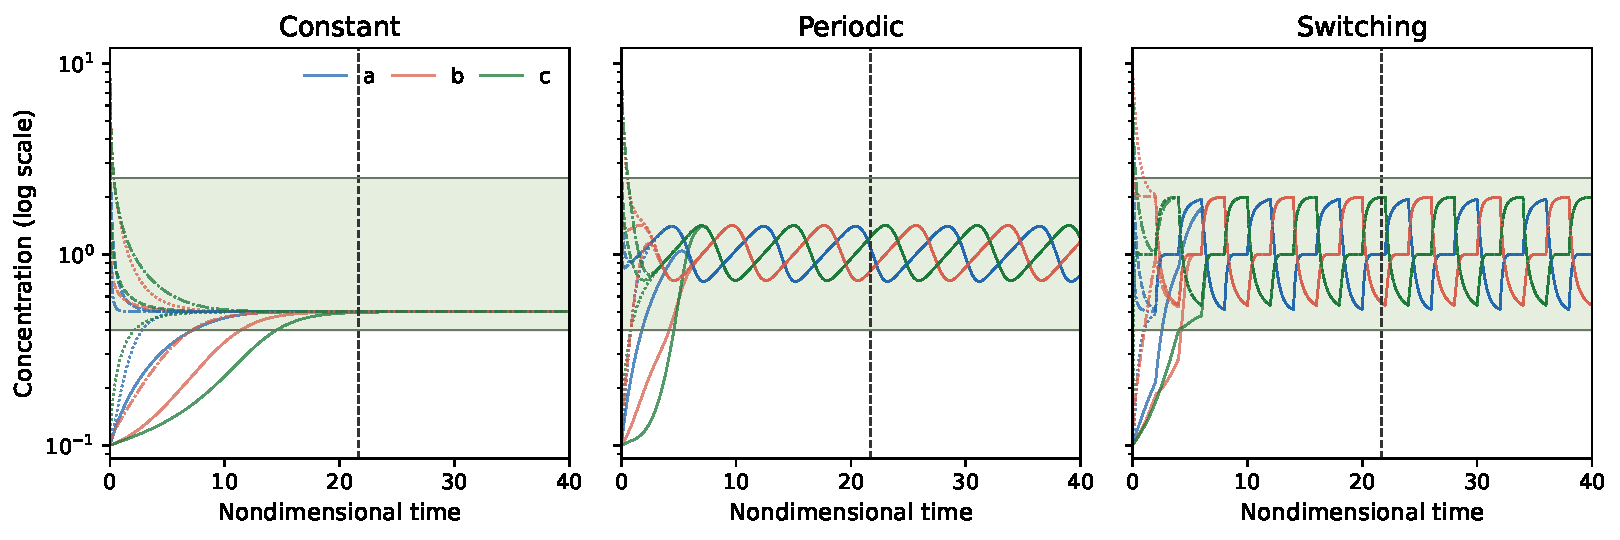
\includegraphics[width=\linewidth]{figures/operating_trajectories.pdf}
\caption{Illustrative trajectories under three declared schedules. The shaded
strip is the proved operating interval $[0.4,2.5]$ for each coordinate and the
dashed line is the staged deadline $347/16$. Colours distinguish $a,b,c$; line
styles distinguish the four startups $(0.1,0.1,0.1)$ (solid), $(10,10,10)$
(dashed), $(0.1,10,0.1)$ (dotted) and $(10,0.1,10)$ (dash-dotted). Constant rates
are $(0.5,2,0.5,2,0.5,2)$; periodic rates are
$k_i(t)=1.25+0.75\sin(2\pi t/8+(i-1)\pi/3)$; switching rates are $0.5$ when
$(\lfloor t/2\rfloor+i-1)\bmod3=0$ and $2$ otherwise, integrated segment by segment
at the exact switching times (SciPy LSODA, relative tolerance $10^{-9}$, absolute
tolerance $10^{-11}$). These simulations illustrate the theorem and supply no
all-history evidence.}
\label{fig:trajectories}
\end{figure}

\subsection{Dimensions and physical reading}\label{sec:dimensions}
Let $A=X_*a$, $B=X_*b$, $C=X_*c$ and $t_{\rm phys}=t_*t$ for declared positive
reference scales. The corresponding physical effective model is
\[
 \dot A=C(q_1-q_2A^2),\qquad \dot B=AB(q_3-q_4B^2),\qquad \dot C=BC(q_5-q_6C^2),
\]
with $k_1=t_*q_1$, $k_2=t_*X_*^2q_2$, $(k_3,k_5)=t_*X_*(q_3,q_5)$ and
$(k_4,k_6)=t_*X_*^3(q_4,q_6)$. The $q_i$ carry different units
($q_1$: time$^{-1}$; $q_2$: concentration$^{-2}$time$^{-1}$; $q_3,q_5$:
concentration$^{-1}$time$^{-1}$; $q_4,q_6$: concentration$^{-3}$time$^{-1}$), so the
common dimensionless box $[1/2,2]^6$ is an assumption on scaled coefficients, not a
statement that unlike physical constants share a numerical range; whether useful
$X_*,t_*$ exist for given measured ranges must be checked case by case. The
physical startup and operating boxes are $[0.1X_*,10X_*]^3$ and $[0.4X_*,2.5X_*]^3$,
and the deadline is $22t_*$; no calibration of $t_*$ is inferred.

The reduced full-rank system is an open, driven effective model. One mass-balanced
bookkeeping realization replaces the forward reactions by
$F_A+C\to A+C$, $F_B+A+B\to A+2B$, $F_C+B+C\to B+2C$ and the backward ones by
$2A+C\to A+C+W_A$, $A+3B\to A+2B+W_B$, $B+3C\to B+2C+W_C$, with maintained feed
reservoirs $F_\bullet$ and removed waste $W_\bullet$ absorbed into the effective
coefficients. Such bookkeeping explains how bounded positive effective coefficients
can be maintained; it does not establish elementary molecular mechanisms,
detailed balance or thermodynamic consistency, and the cubic terms should be read
as effective cooperative kinetics. Retention of all species in a positive box
implies neither net useful production nor the absence of futile cycles, and it is
a deterministic guarantee, not a statement about finite-copy stochastic extinction.

\section{Formal verification and reproducibility}\label{sec:formal}

The scientific development uses Lean~4 (\lean{leanprover/lean4:v4.30.0}) and
Mathlib commit \lean{c5ea00351c28e24afc9f0f84379aa41082b1188f}. Historical
source bytes and receipts are preserved. Fresh additive checks on October~8,
2026 reuse exactly matching historical dependency artifacts; they compile the
new modules and check the new roots. Warnings are errors and every selected
root reports only \lean{propext}, \lean{Classical.choice} and \lean{Quot.sound}.
This scientific verification is distinct from migration and mechanical
verification of a Palomar submission.

The affine construction (Lemma~\ref{lem:affine}) is ported from the public Lean
sources of~\cite{OpenAI2026Boundedness,OpenAI2026Uniform}, at the cited commit,
into \lean{proofs/EndotacticPermanence/Imported/}. The relevant declarations
\lean{OAI.Problem326.Affine.exists_fullCertificate} and
\lean{FullCertificate.uniform_activity} have no weak-reversibility hypothesis.
The proofs and upstream hashes are included; no fixed-point or geometric axiom
was added.

\paragraph{The fresh roots.}
The signed model has a finite reaction index $R$ with source and target maps
$R\to\texttt{Fin d}\to\R$. Its \lean{Endotactic} is Definition~\ref{def:endo},
testing every real direction. \lean{PositiveRateBox} has positive lower bounds
and coordinatewise upper bounds. \lean{AEAdmissible} means coordinatewise
a.e. measurability and a.e. box membership for Lebesgue measure restricted to
$[0,\infty)$. \lean{IsCaratheodorySolution} is exactly initial data, absolute
continuity on every $[0,T]$, and the vector ODE a.e. on $(0,T)$.

In the namespace \lean{EndotacticPermanence.RealComplex},
\lean{endotactic_permanence_compact_ae}
(\lean{Real/AlmostEverywherePermanence.lean}) proves Theorem~\ref{thm:main} in
this signed domain. Its quantifier order is
$\exists K\;\forall Q\;\exists T_Q\;\forall x_0\in Q\;\forall k$.
It concludes global positive existence, class preservation, absorption,
uniqueness among positive solutions, and invariance for every positive solution
starting in $K$. The pointwise-rate root is
\lean{RealComplex.endotactic_permanence_compact}. Positive-box regularity and
clamped-field existence replace ambient polynomial regularity; uniqueness
uses finite-time positive box enclosures.

\lean{RealComplex.mass_action_continuous_dependence_ae}
(\lean{Real/ContinuousDependence.lean}) proves Proposition~\ref{prop:dependence}
with its Lipschitz constant chosen before the history and curves.
\lean{EndotacticPermanence.repair_rate_history} constructs a common null-set
repair, and \lean{caratheodory_solution_congr_forward_ae} transfers the solution
predicate for every curve. The fresh natural-complex root
\lean{EndotacticPermanence.endotactic_permanence_compact_ae} additionally
preserves the historical theorem's ambient uniqueness conclusion.

\begin{table}[ht]
\centering\small
\renewcommand{\arraystretch}{1.15}
\begin{tabular}{p{0.60\linewidth}p{0.34\linewidth}}
\toprule
Result & Verification status\\
\midrule
Signed real-complex permanence, a.e. admissible histories: global positive
solutions, positive-solution uniqueness, invariant compact convex $K$,
compact-initial uniform deadline & Fresh strict Lean root\\
Natural-complex permanence with a.e. rates and ambient uniqueness
& Fresh strict Lean root\\
Initial-data continuous dependence on a compact positive region, signed
complexes and a.e. rates & Fresh strict Lean root\\
Natural-complex pointwise-rate roots and continuous dependence
& Preserved historical checks\\
Feedback, periodic operation and autonomous equilibria
& Conventional proofs\\
Example: classification, invariant boxes, clock construction, Riccati comparison
& Conventional proofs\\
Example: clocked comparisons, inverse-square transformation, two-stage clock
floors and exact roundings & Preserved historical checks\\
\bottomrule
\end{tabular}
\caption{Formal and conventional scope. No conditional fixed-point statement
is counted as a proved corollary.}
\label{tab:formal}
\end{table}

\paragraph{Example correspondence.}
The historical \lean{RecoveryComparison.lean} checks clocked comparisons,
the inverse-square transformation, two-stage clock floors and coordinate recovery.
Its principal composed declaration is \lean{staged_coordinate_recovery},
with applications \lean{staged_recovery_second} and \lean{staged_recovery_third}.
The exact roundings are \lean{a_stage_deadline_lt_nine},
\lean{recovery_deadline_lt_38} and \lean{staged_deadline_lt_22}.
These remain conditional on the explicitly listed curve and clock hypotheses
in Section~\ref{sec:comparisons}.

\paragraph{Remaining formal boundaries.}
Periodic and equilibrium corollaries require a finite-dimensional fixed-point
theorem and its solution-map interfaces. Feedback needs a local closed-loop
existence and continuation proof. Those results, and the fixture-specific
invariance and Riccati comparisons, are conventional here. They are not part
of the compared formal claim. No custom axiom was introduced to close them.

\paragraph{Reproduction.}
The accompanying repository includes the manuscript sources, bibliography,
figures, figure producer and saved trajectory data, together with the Lean
development migrated to Lean~4.35.0-rc2. The independent statement in
\lean{Challenge.lean} and its implementation in \lean{Solution.lean} select
uniform permanence and initial-data continuous dependence. Both declarations
passed local Comparator and all six bundled kernel checks. The report
\lean{verification/local-check.json} records the exact source hashes, checked
declarations and an extract of the saved results. These checks are separate
from the scientific Lean~4.30.0 checks described above. Build instructions are
in \lean{BUILD.md}; pinned upstream attribution is in
\lean{UPSTREAM_PROVENANCE.json}. The additional corollaries retain the formal
and conventional scope stated in Table~\ref{tab:formal}.

\section{Limits and open questions}\label{sec:limits}

The theorem permits arbitrary measurable switching inside a fixed positive compact
box, and its constants depend on that box; neither bound can simply be dropped.
For the endotactic pair $A\rightleftarrows2A$ with common history
$k_+(t)=k_-(t)=e^{-t}$, the operational clock has finite total length and the
logistic solution satisfies $a(t)\le e\,a_0$, so arbitrarily small startups never
reach a common positive floor. For $0\rightleftarrows A$ with birth rate $1+t$ and
death rate $1$, $a'=1+t-a$ grows without bound. These examples delimit the
hypothesis; they do not weaken the classwise statement under it.

The construction supplies a finite sum of barrier delays, not an efficient
algorithm; making the affine data effective, and extracting network-specific
recovery constants of the kind obtained in Section~\ref{sec:example}, are
quantitative problems. The staged argument there illustrates a general principle
that may deserve a theorem of its own: a recovered component accelerates the
guaranteed recovery of the components it drives, without any reduction of the
rate uncertainty, provided the dependency order is respected. Positive
deterministic permanence says nothing by itself about extinction in finite
stochastic populations; periodic-solution existence leaves stability,
entrainment and uniqueness open; and the feedback proposition requires its local
hypotheses. Which quantitative conclusions survive as a lower rate bound tends to
zero, and under what monotonicity conditions periodic existence becomes
entrainment, are natural next questions.

\appendix
\section{Lean statement of the signed root}\label{app:lean}
The fresh compact-initial root is reproduced below, transliterated from Unicode
to ASCII. Its namespace is \lean{EndotacticPermanence.RealComplex};
\lean{AEAdmissible} is defined in Section~\ref{sec:formal}. The source file and
the elaborated declaration in its receipt are authoritative. The preserved
natural-complex statements remain included in the source bundle.
{\scriptsize\begin{verbatim}
theorem endotactic_permanence_compact_ae {d : Nat} {R : Type*} [Fintype R]
    (source target : R -> Fin d -> Real)
    (endo : Endotactic source target) (B : PositiveRateBox R)
    (c : Fin d -> Real) (hc : PositiveState c) :
    exists K : Set (Fin d -> Real), K.Nonempty /\ IsCompact K /\ Convex Real K /\
      K subset positiveClass source target c /\
      (forall Q : Set (Fin d -> Real), IsCompact Q -> Q subset positiveClass source
        target c ->
        exists T : Real, 0 <= T /\ forall x0 in Q, forall k : Real -> R -> Real,
          AEAdmissible B k -> exists x : Real -> (Fin d -> Real),
            IsCaratheodorySolution (fun t => indexedMassAction source target (k t)) x0 x
              /\
            (forall t : Real, 0 <= t -> x t in positiveClass source target c) /\
            (forall t : Real, T <= t -> x t in K) /\
            (forall y : Real -> (Fin d -> Real),
              IsCaratheodorySolution (fun t => indexedMassAction source target (k t)) x0
                y -> (forall t : Real, 0 <= t -> PositiveState (y t)) ->
                EqOn x y (Ici 0))) /\
      (forall x0 in K, forall k : Real -> R -> Real, AEAdmissible B k ->
        forall x : Real -> (Fin d -> Real),
          IsCaratheodorySolution (fun t => indexedMassAction source target (k t)) x0 x
            -> (forall t : Real, 0 <= t -> PositiveState (x t)) ->
          forall t : Real, 0 <= t -> x t in K)
\end{verbatim}}

\bibliographystyle{plain}
\bibliography{refs}
\end{document}
